\documentclass[10pt,sans,usenames,dvipsnames,french,compress]{beamer}

\usepackage[french]{babel}
\usepackage[utf8]{inputenc}
\usepackage[T1]{fontenc}
\usepackage{lmodern}
\usepackage{graphicx}
\usepackage[absolute,overlay]{textpos}
\usepackage{dirtree}
\usepackage{listings}

\mode<presentation>

\usetheme{Warsaw}
\useoutertheme[subsection=false]{miniframes}

% Fix the crop bullets in the headline
\makeatletter
\setbeamertemplate{headline}
{
  \vskip-0.8ex
  \begin{beamercolorbox}{section in head/foot}
  \vskip2pt\insertnavigation{\paperwidth}\vskip4pt
  \end{beamercolorbox}%
}
\makeatother

%infolines footer
\defbeamertemplate*{footline}{infolines theme}
{
	\leavevmode%
	\hbox{%
	\begin{beamercolorbox}[wd=.333333\paperwidth,ht=2.25ex,dp=1ex,center]{author in head/foot}%
	 \usebeamerfont{author in head/foot}\insertshortauthor%~~(\insertshortinstitute)
	\end{beamercolorbox}%
	\begin{beamercolorbox}[wd=.333333\paperwidth,ht=2.25ex,dp=1ex,center]{title in head/foot}%
	 \usebeamerfont{title in head/foot}\insertshorttitle
	\end{beamercolorbox}%
	\begin{beamercolorbox}[wd=.333333\paperwidth,ht=2.25ex,dp=1ex,right]{date in head/foot}%
	 \usebeamerfont{date in head/foot}\insertshortdate{}\hspace*{2em}
	 \insertframenumber{} / \inserttotalframenumber\hspace*{2ex}
	\end{beamercolorbox}}%
	\vskip0pt%
}

% Terminal-like listing formatting
\lstdefinestyle{Term}
{
    backgroundcolor=\color{black},
    basicstyle=\scriptsize\color{white}\ttfamily,
    gobble=22
}

\graphicspath{{images/}}

\setbeamersize{text margin left=15pt,text margin right=15pt}

% Disable navigation icons
\beamertemplatenavigationsymbolsempty

% Titlepage
\title{CTF SeCReTS}
\subtitle{Présentation}
\author{Alexis Brouste -- Loïc Martin -- Alizée Murat}
\date{Mercredi 20 mars 2019}
\institute[UVSQ]{UVSQ}

% See for colors names: https://en.wikibooks.org/wiki/LaTeX/Colors

\begin{document}

\section{Introduction}
\subsection{Page de titre}
\begin{frame}[plain]
	\titlepage
\end{frame}

\subsection{Défis présentés}
\begin{frame}{Défis présentés}
	\begin{itemize}
		\item 114 - Reversing 3
		\item 118 - WPA forensics
		\item 120 - Courbe elliptique et AES-CCM
	\end{itemize}
\end{frame}

\section{114 - Reversing 3}
\subsection{Titre}
\begin{frame}
	\begin{beamercolorbox}[sep=8pt,center]{title}
		\usebeamerfont{title}{114 - Reversing 3}
	\end{beamercolorbox}
\end{frame}

\section{118 - WPA forensic}
\subsection{Titre}
\begin{frame}
	\begin{beamercolorbox}[sep=8pt,center]{title}
		\usebeamerfont{title}{118 - WPA forensic}
	\end{beamercolorbox}
\end{frame}

\subsection{Découverte}
\begin{frame}
	\begin{block}{Fichiers}
		\begin{small}
			\dirtree{%
				.1 118-wpa-forensics/.
				.2 indice.txt.
				.2 README.txt.
				.2 {\color<3->{OliveGreen}psk-01.cap}.
			}
		\end{small}
	\end{block}

	\begin{block}<2->{\textit{indice.txt}}
		\begin{itshape}	
			\begin{small}
				In the ennemy base, there is a building, which is guarded by hundreds of 
				highly trained soldiers.

				In this building, there is a WPA-PSK protected wifi with an unbreakable
				password, like {\color<3->{Dandelion}a 10 letter english word (all uppercase) followed by 2
				digits}.

				In this wifi network, there is a web server that only the flag keeper
				(=admin) may access.

				{\color<3->{Dandelion}The flag is his password}

				Good luck!

				PS: By the way, a geek visitor just told me he was walking around 
				the base with his linux laptop (of course, his wlan interface was 
				in  monitor-mode by default). Anyways, he gave me this capture:
				{\color<3->{OliveGreen}psk-01.cap}
			\end{small}
		\end{itshape}
	\end{block}
\end{frame}

\subsection{Procédure}
\begin{frame}{Procédure}
	\begin{itemize}
		\item Déchiffrement du trafic
		\begin{itemize}
			\item Génération de dictionnaire
			\item Cassage par force-brute de la clef WPA
		\end{itemize}
		\item Analyse du trafic
		\begin{itemize}
			\item Récupération du drapeau
		\end{itemize}
	\end{itemize}
\end{frame}

\subsection{Déchiffrement}
\subsubsection{Création de dictionnaire}
\subsubsection{Cassage de la clef WPA}
\begin{frame}[fragile]{Cassage de la clef WPA}
	\begin{block}{Outil : Aircrack}
		\begin{lstlisting}[style=Term]
			~# aircrack-ng -w generated_dict.txt psk-01.cap
		\end{lstlisting}
	\end{block}

	\begin{block}{Cassage en cours}<2->
		\begin{figure}
			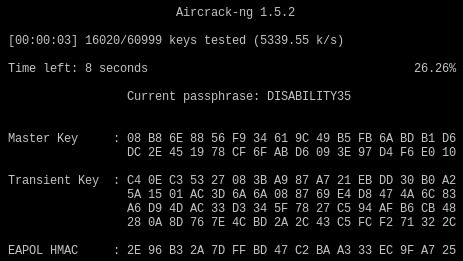
\includegraphics[width=0.7\linewidth]{118/aircrack0}
		\end{figure}
	\end{block}
\end{frame}

\begin{frame}{Cassage de la clef WPA}
	\begin{block}{Succès}
		\begin{figure}
			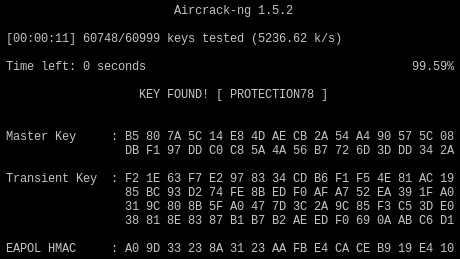
\includegraphics[width=0.7\linewidth]{118/aircrack1}
		\end{figure}
	\end{block}

	\begin{exampleblock}<2->{En bref}
		\begin{itemize}
			\item Clef : \textbf{PROTECTION78}
			\item<3-> Importance d'un dictionnaire optimisé (cassage en onze secondes !)
		\end{itemize}
	\end{exampleblock}
\end{frame}


\subsection{Analyse du trafic}


\section{120 - Courbe elliptique et AES-CCM}
\subsection{Titre}
\begin{frame}
	\begin{beamercolorbox}[sep=8pt,center]{title}
		\usebeamerfont{title}{120 - Courbe elliptique et AES-CCM}
	\end{beamercolorbox}
\end{frame}

\end{document}
